\secnumbersection{VALIDACIÓN DE LA SOLUCIÓN}

\subsection{Algoritmo}

El algorimo final sigue el flujo detallado en el Anexo 3, el cuál fue detallado en el Capítulo 3. El mismo se divide en los siguientes pasos:

\subsubsection{Log Formatting}
Cumple con el proceso planteado en la sección 3.3.1, donde se remueven los tokens de fecha y hora iniciales, debido a su redundancia a nivel de línea, además de corregir otros detalles de formato con tal de facilitar el posterior análisis.

\subsubsection{Obs Filtering} 
Cumple con el proceso descrito en la sección 3.3.2, donde se obtiene un archivo csv con las observaciones de la noche seleccionada, para luego formar bloques de tiempo basados en los tiempos que tarda cada observaciones, más el efecto de parámetros de margen y unión, donde finalmente se filtran las líneas de log con tal de quedar solo con aquellas cuya fecha se encuentre dentro de alguno de esos bloques de tiempo.

\subsubsection{Log Parsing}
Cumple con el proceso descrito en la sección 3.4, donde a base de una archivo plano de plantillas, se itera sobre las líneas de log, aplicando cada plantilla por línea hasta encontrar alguna que calze y guardar la data extraída en un json final.

Como se mencionó en la sección 3.4.2, el método para realizar la extracción es mediante Expresiones Regulares, lo cuál se manifiesta tanto en el archivo de plantillas que se ingresa a la función, junto con las líneas a extraer, como en el método de extracción que se aplica a línea de log.

\subsubsection{Generate Dataframes} 
Cumple con el proceso de la sección 3.5.2, donde se menciona el traslado de los datos del json generado en la función anterior a un conjunto de dataframes, usando los campos \"group\" y \"label\" como etiquetas para reconocer a qué dataframe destinar los datos.

De esta función se generan 4 dataframes, como se señalo en la sección 3.5.1: df\_corrections, para las instancias de corrección; df\_images, para las imágenes capturadas; df\_f\_dist, para las distribuciones de fuerza de los actuadores; y df\_additional\_data, para los datos adicionales relacionados con la Óptica Activa.

\subsubsection{Validate Forces} 
Cumple con el segundo item de la sección 3.5.3, donde se especifica la validación de los datos dentro de df\_f\_dist generado en la función anterior. 

Principalmente, se eliminan los datos con ID nulo, además de remover aquellos que no sean antecedidas y/o seguidas por imágenes únicas.

\subsubsection{Validate Images} 
Cumple con el tercer item de la sección 3.5.3, donde se especifica la validación de los datos dentro de df\_images generado en la función anterior. Solamente se eliminan aquellos datos con ID nulo.

\subsubsection{Link Images} 
Cumple con el requisito de la sección 3.5.1, sobre df\_images manteniendo la dirección local del archivo .fits correspondiente como un atributo de los datos del dataframe.

En esta función, se ingresa a la carpeta donde estan almacenados los archivos .fits, se extrae el número de ID y el tiempo de exposición del header de cada .fits y se usan estos para buscar el dato de df\_images que le sea correspondiente. En caso de encontrarlo, se guarda su dirección local en el atributo correspondiente del dato.

\subsubsection{Validate Corrections} 
Cumple con el primer item de la sección 3.5.3, donde se especifica la validación de los datos dentro de df\_corrections generado en la función anterior.

Principalmente se eliminan los datos con ID nulo, además de remover aquellos sin distribución de fuerza posterior a la corrección.

\subsubsection{Link Dataframes}
Cumple con el proceso descrito en la sección 3.5.4, en la que se indica como calzar los datos de un dataframe con los datos de dataframe df\_corrections mediante los timestamp de estos datos, comparando estos para luego copiar la ID del dato de la cantidad deseada en un campo designado dentro del dato correspondient en df\_corrections.

Para esta función, como la construcción de relaciones entre df\_images con df\_corrections y entre df\_f\_dist con df\_corrections es identico, por lo que se pudo generalizar y paramétrizar esta construcción en una misma función, que varía con el dataframe de la cualidad deseada, el nombre de la cualidad deseada y el campo de tiempo dentro del dataframe, como parámetros de entrada.

\subsection{Ejecución}

Para ejecutar el código desarrollado, se debe entregar la fecha y el número del UT, en ese orden, del registro a analizar. Para el apropiado funcionamiento del algoritmo, el archivo de log debe estar previamente cargado en el sistema local.

Además se desarrolló un sistema de flags opcionales que otorga la posibilidad de habilitar o deshabilitar las funciones descritas en la sección 4.2.1.

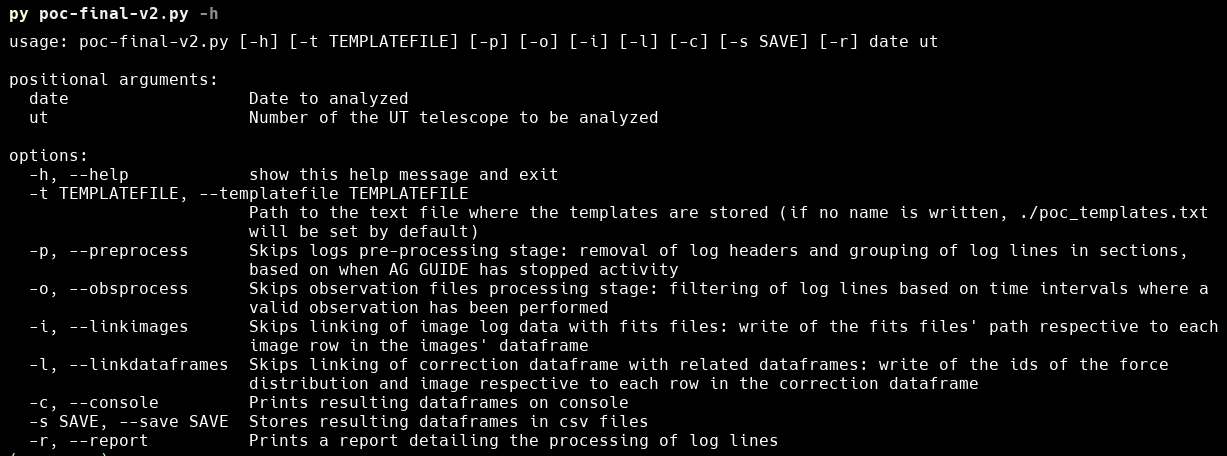
\includegraphics[width=12cm,height=8cm]{figures/flags.png} \\

Existen 2 posibles modos de retorno de los dataframes generados: por consola o por csv. Estos se habilitan con las flags -c y -s, respectivamente.

\subsection{Pruebas}

Para corroborar el correcto funcionamiento del algoritmo, es necesario analizar los resultados del mismo, junto con revisar el rendimiento y exactitud de la ejecución.

\subsubsection{Metodología}

Para poder analizar el desempeño y resultados del algoritmo, primero se realiza un conteo manual de las instancias de corrección, las distribuciones de fuerza y las imagenes presenten en una muestra de archivos de log. Luego, se ejecuta el algoritmo para procesar los mismos archivos de log, y se comparan los resultados. 

La muestra se compone de los siguientes archivos de log:

\begin{itemize}
    \item L1 : Archivo de log para la observación del UT 1 durante la noche del 4 de Agosto del 2025.

    \item L2 : Archivo de log para la observación del UT 1 durante la noche del 5 de Agosto del 2025.

    \item L3 : Archivo de log para la observación del UT 3 durante la noche del 4 de Agosto del 2025.

    \item L4 : Archivo de log para la observación del UT 3 durante la noche del 5 de Agosto del 2025.

    \item L5 : Archivo de log para la observación del UT 4 durante la noche del 4 de Agosto del 2025.

    \item L6 : Archivo de log para la observación del UT 4 durante la noche del 5 de Agosto del 2025.    
\end{itemize}

Una vez realizadas las ejecuciones, se procede a analizar las estadísticas de los resultados, más específicamente el número de instancias de corrección, distribución de fuerzas e imágenes obtenidas, además del tiempo de ejecución.

Este proceso de revisión se realizará primero en ámbitos generales del algoritmo, y luego se revisará para cada etapa de forma más específica.

\subsubsection{Resultados generales}

Los resultados encontrados de forma manual para cada archivo de log se refleja en la Tabla \ref{table:manual}. Luego, las cantidades encontradas en los mismos archivos por el algoritmo se encuentran en la Tabla \ref{table:auto}.


\begin{table}[h]
    \centering
    \caption{\label{table:manual} Cantidades encontradas de forma manual}
    \begin{tabular}{|p{2.8cm}|p{2.8cm}|p{2.8cm}|p{2.8cm}|p{2.8cm}|}
        \hline
        Log & N° de líneas & N° de correcciones & N° de dist. de fuerza & N° de imágenes \\
        \hline
        L1 & 427195 & 626 & 586 & 851 \\
        \hline
        L2 & 384729 & 598 & 562 & 802 \\
        \hline
        L3 & 409830 & 537 & 277 & 908 \\
        \hline
        L4 & 371450 & 546 & 262 & 741 \\
        \hline
        L5 & 444126 & 491 & 287 & 786 \\
        \hline
        L6 & 422312 & 495 & 358 & 713 \\
        \hline
    \end{tabular}
\end{table}


\begin{table}[h]
    \centering
    \caption{\label{table:auto} Cantidades encontradas por el algoritmo}
    \begin{tabular}{|p{2.3cm}|p{2.3cm}|p{2.3cm}|p{2.3cm}|p{2.3cm}|p{2.3cm}|}
        \hline
        Log & N° de líneas & N° de correcciones & N° de dist. de fuerza & N° de imágenes & Tiempo (en segundos) \\
        \hline
        L1 & 427195 & 4 & 5 & 11 & 61.92 \\
        \hline
        L2 & 384729 & 31 & 33 & 54 & 89.33 \\
        \hline
        L3 & 409830 & 4 & 5 & 8 & 69.49 \\
        \hline
        L4 & 371450 & 19 & 19 & 46 & 79.14 \\
        \hline
        L5 & 444126 & 3 & 3 & 4 & 59.18 \\
        \hline
        L6 & 422312 & 18 & 18 & 31 & 103.25 \\
        \hline
    \end{tabular}
\end{table}

Es evidente la amplia diferencia entre ambas cantidades, sin embargo, existen motivos para explicarlo.

Primero, se debe mencionar que la extracción manual se realizó mediante un simple conteo de lineas de log según ciertos tokens clave, mientras que para la extracción con el algoritmo se aplicó lógica durante las validaciones y filtros que permiten un conteo con información más certera, aunque reducida en tamaño.

Ejemplos de reglas incumplidas en los logs: se ha visto que en los registros de log, existen varias fotos que se pueden tomar consecutivamente en lapsos de unos pocos segundos; distribuciones de fuerza que no son anticipados ni seguidos directamente por una toma de imágen; entre otros. Estos casos, son detectados por el algoritmo, evitando la extracción de estos datos extra.

El otro motivo de porque la diferencia en el número de cantidades es la filtración por observación: la cantidad de observaciones totales es baja, lo cuál inmediatamente deja fuera a una buena parte de las cantidades presentes en el archivo de log, como se puede ilustrar en la siguiente imágen:

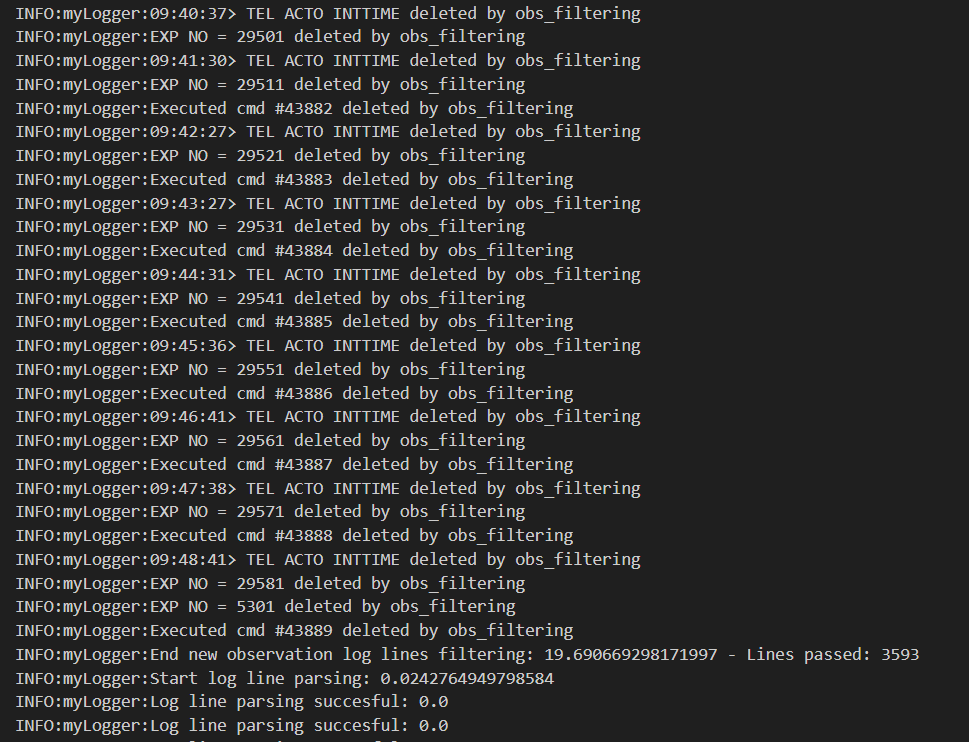
\includegraphics[width=13.5cm,height=9cm]{figures/log_deletes.png} \\

En la imágen anterior, los nombres mostrados equivalen a líneas de imágen, desechadas de la extracción final, debido a no calzar con algún horario de observación.

Ahora bien, como se menciono en la sección 3.3.2, el filtro de observaciones se realiza con tres parámetros, los cuáles son de asignación directa dentro del código. Por ende, la modificación de estos parámetros ampliaría el rango de búsqueda de las cantidades en el archivo de log. Actualmente, se definieron los margenes anterior y posterior como 10 segundos cada uno, y el umbral de unidad de los bloques de observación se encuentra en 30 segundos.

Es posible aumentar estos paramétros, sin embargo tampoco se pueden llegar a extremos muy altos que terminen volviendo obsoleto al proceso de filtro por observación.

\subsection{Resultados para Filtrado de líneas de log}

Parte crucial de este etapa es el cruce de los registros de log con los datos de observaciones, con tal de filtrar los primeros, tal como se explicó en la sección 3.4.2. Con esto en mente, se puede examinar el rendimiento de esta etapa comparando la cantidad de líneas de log que ingresa con la cantidad que sale, para cada uno de los casos descritos al inicio de esta sección.

Los resultados de estas pruebas se exponen en la Tabla \ref{table:etapa1}


\begin{table}[h]
    \centering
    \caption{\label{table:etapa1} Cantidad de líneas de log filtradas}
    \begin{tabular}{|p{3.5cm}|p{3.5cm}|p{3.5cm}|p{3.5cm}|}
        \hline
        Log & N° de líneas entrada & N° de líneas salida & P. de reducción \\
        \hline
        L1 & 427195 & 3829 & 99.10\% \\
        \hline
        L2 & 384729 & 23475 & 93.90\% \\
        \hline
        L3 & 409830 & 4496 & 98.90\% \\
        \hline
        L4 & 371450 & 22048 & 94.06\% \\
        \hline
        L5 & 444126 & 3593 & 99.19\% \\
        \hline
        L6 & 422312 & 27365 & 93.52\% \\
        \hline
    \end{tabular}
\end{table}

Se puede notar de inmediato la efectividad de los filtros aplicados en esta etapa: en todos los casos probados se redujo el número de líneas de log en más de un 90\%.

Esta eficiencia trae ventajas y desventajas: por un lado, se asegura que las líneas de log que pasen a la etapa de Extracción de Datos correspondan a observaciones válidas del telescopio; por el otro lado, es posible teorizar que se están desechando líneas de log que puedan poseer información relacionada con la ejecución del sistema de Óptica Activa.

\subsection{Resultados para Extracción de los datos}

Se prueban los dos métodos de extracción mencionados en la sección 3.4.2, usando la serie de parámetros iniciales señalados en el inicio, y se registran los tiempos y cantidad de datos extraídos para cada método:

\begin{table}[h]
    \centering
    \caption{\label{table:etapa2} Tiempos y cantidad de datos para modos de extracción}
    \begin{tabular}{|p{2cm}|p{3cm}|p{3cm}|p{3cm}|p{3cm}|}
        \hline
        Log & N° de datos TTP & Tiempo TTP (en segundos) & N° de datos Regex & Tiempo Regex (en segundos) \\
        \hline
        L1 & 64 & 156.56 & 68 & 61.92 \\
        \hline
        L2 & 533 & 636.70 & 546 & 89.33 \\
        \hline
        L3 & 59 & 138.05 & 62 & 69.49 \\
        \hline
        L4 & 441 & 569.63 & 450 & 79.14 \\
        \hline
        L5 & 31 & 144.02 & 34 & 59.18 \\
        \hline
        L6 & 462 & 710.65 & 473 & 103.25 \\
        \hline
    \end{tabular}
\end{table}

Con esta prueba, se puede notar que ambos métodos de extracción retornan cantidades similares de datos, sin embargo TTP toma una mayor cantidad de tiempo en comparación con Regex. Con esto, se corrobora que el método de extracción con Regex es más apropiado para el algoritmo.

Una vez determinado el método de extracción, se procede a determinar la cantidad de líneas cuyos datos fueron extraídos sobre la cantidad de líneas que ingresaron a la etapa, similar a la prueba realizada para Filtrado de Líneas de Log. Los resultados se muestran en la Tabla \ref{table:etapa2c2}

Esto se revisa en esta etapa porque, si bien aquí no tiene el fin de filtrar directamente, esto igualmente ocurre frecuentemente debido a la aplicación de plantillas, donde aquellas líneas de log que no calzen con ninguna plantilla serán descartadas.


\begin{table}[h]
    \centering
    \caption{\label{table:etapa2c2} Cantidad de líneas de log extraídas}
    \begin{tabular}{|p{3.5cm}|p{3.5cm}|p{3.5cm}|p{3.5cm}|}
        \hline
        Log & N° de líneas entrada & N° de líneas salida & P. de reducción \\
        \hline
        L1 & 3829 & 135 & 96.47\% \\
        \hline
        L2 & 23475 & 940 & 95.99\% \\
        \hline
        L3 & 4496 & 142 & 96.84\% \\
        \hline
        L4 & 22048 & 819 & 96.29\% \\
        \hline
        L5 & 3593 & 73 & 97.97\% \\
        \hline
        L6 & 27365 & 806 & 97.05\% \\
        \hline
    \end{tabular}
\end{table}


Según lo reflejado en la Tabla \ref{table:etapa2c2}, los porcentajes de reducción son incluso mayores que en la etapa anterior, donde no bajan del 95\%.

Sin embargo, a diferencia de la etapa anterior, estos porcentajes altos no comprometen la cantidad de datos extraídos; por el contrario, son un sintoma esperable del proceso de aplicación de plantillas.

Para ilustrar esta defensa, se analizan los logs de operación del algoritmo, donde se destacan campos desechados durante la etapa de extracción. Los resultados para cada caso se presenta en la Tabla \ref{table:etapa2c3}.


\begin{table}[h]
    \centering
    \caption{\label{table:etapa2c3} Perdidas de datos durante extracción}
    \begin{tabular}{|p{3.5cm}|p{3.5cm}|p{3.5cm}|p{3.5cm}|}
        \hline
        Log & I. de corrección perdidas & Dist. de fuerzas perdidas & Imágenes perdidas \\
        \hline
        L1 & 2 & 0 & 0 \\
        \hline
        L2 & 2 & 0 & 0 \\
        \hline
        L3 & 3 & 0 & 0 \\
        \hline
        L4 & 20 & 0 & 0 \\
        \hline
        L5 & 0 & 0 & 0 \\
        \hline
        L6 & 17 & 0 & 0 \\
        \hline
    \end{tabular}
\end{table}

Incluso para el caso de L4 y L6, donde se pierden más datos en la tabla, son cantidades menores en comparación a los datos que extraen exitosamente (referidos en la Tabla \ref{table:etapa2}).

\subsection{Resultados para Guardado de los datos}

Similar a las etapas anteriores, se va a comparar la cantidad de datos que entran a la etapa con la cantidad de datos que salen de la misma. 

Solo se contarán datos de dsitribución de fuerzas, instancias de corrección e imágenes tomadas. Esto porque en esta etapa se realizan validaciones que pueden eliminar datos dependiendo del contexto, y dichas validaciones solo se aplican a esos tipos de datos.

Los resultados de este análisis se presentan en la Tabla \ref{table:etapa3}


\begin{table}[h]
    \centering
    \caption{\label{table:etapa3} Cantidad de datos filtrados}
    \begin{tabular}{|p{3.5cm}|p{3.5cm}|p{3.5cm}|p{3.5cm}|}
        \hline
        Log & N° de datos entrada & N° de datos salida & P. de reducción \\
        \hline
        L1 & 26 & 20 & 30\% \\
        \hline
        L2 & 146 & 118 & 19.18\% \\
        \hline
        L3 & 24 & 18 & 25\% \\
        \hline        
        L4 & 116 & 84 & 27.59\% \\
        \hline
        L5 & 14 & 10 & 40\% \\
        \hline
        L6 & 100 & 67 & 33\% \\
    \end{tabular}
\end{table}

Si bien presenta bajas enlos números de datos, son porcentajes menores a los presentes en las etapas anteriores. Es posible que estas bajas sean causados por las validaciones, como se menciono anteriormente, considerando que en dichas validaciones se remueven valores con nulidad o que no cumplan con el orden distribución de fuerza - imágen establecido.